\documentclass[]{article}

\usepackage{parskip,amsmath,graphicx}
\usepackage[margin=0.5in]{geometry}
\usepackage[section]{placeins}
\usepackage{pdfpages}

%opening
\title{Midterm - ASE 389P.8 Satellite Control Systems}
\author{Corey Marcus}

\begin{document}

\maketitle

\newcommand{\CrossProd}[1]{\left[ #1 \times \right]}

\section{Part 1}

\begin{figure}[!h]
	\centering
	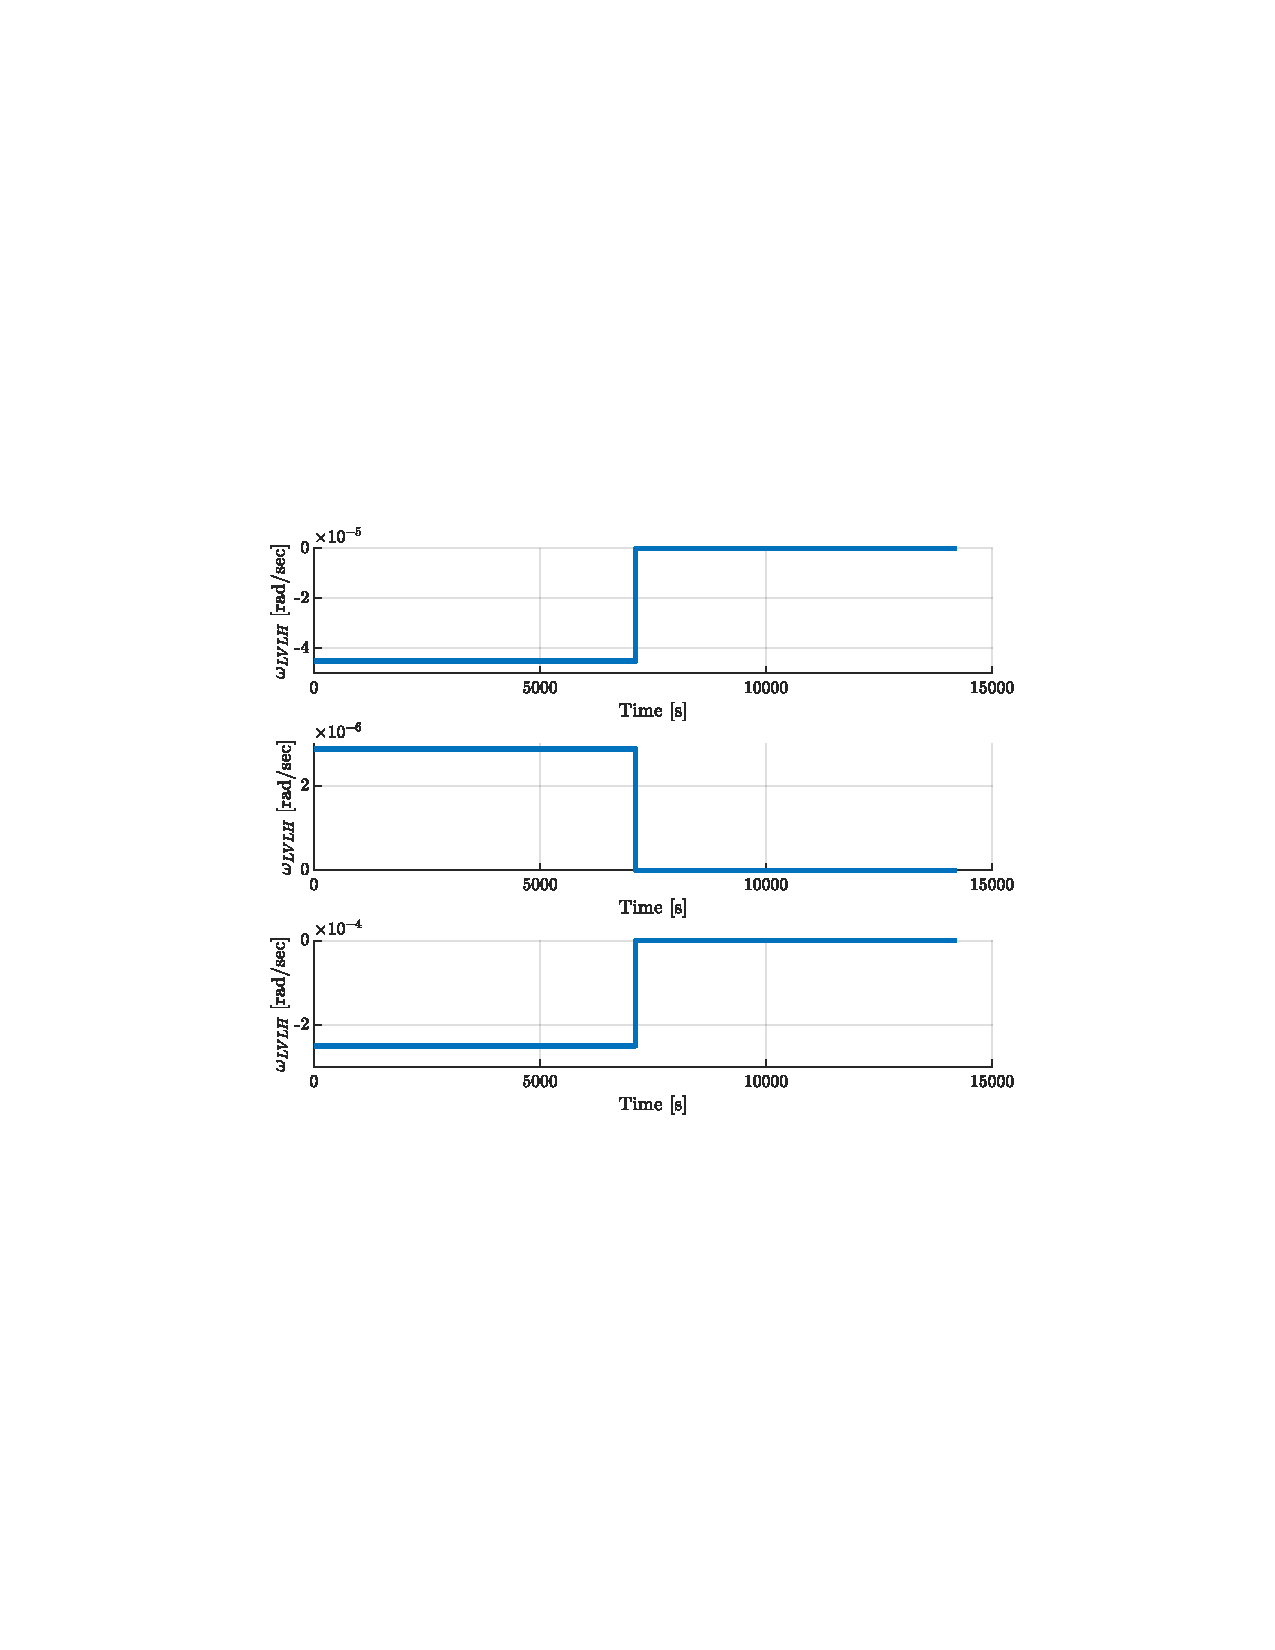
\includegraphics[width=\linewidth,trim={4cm, 8cm, 4cm, 8cm},clip]{figs/P1Q1.pdf}
	\caption{The nominal LVLH to body angular rates. We begin with a constant rate maneuver, followed by a LVLH hold.}
	\label{fig:P1Q1}
\end{figure}

\begin{figure}[!h]
	\centering
	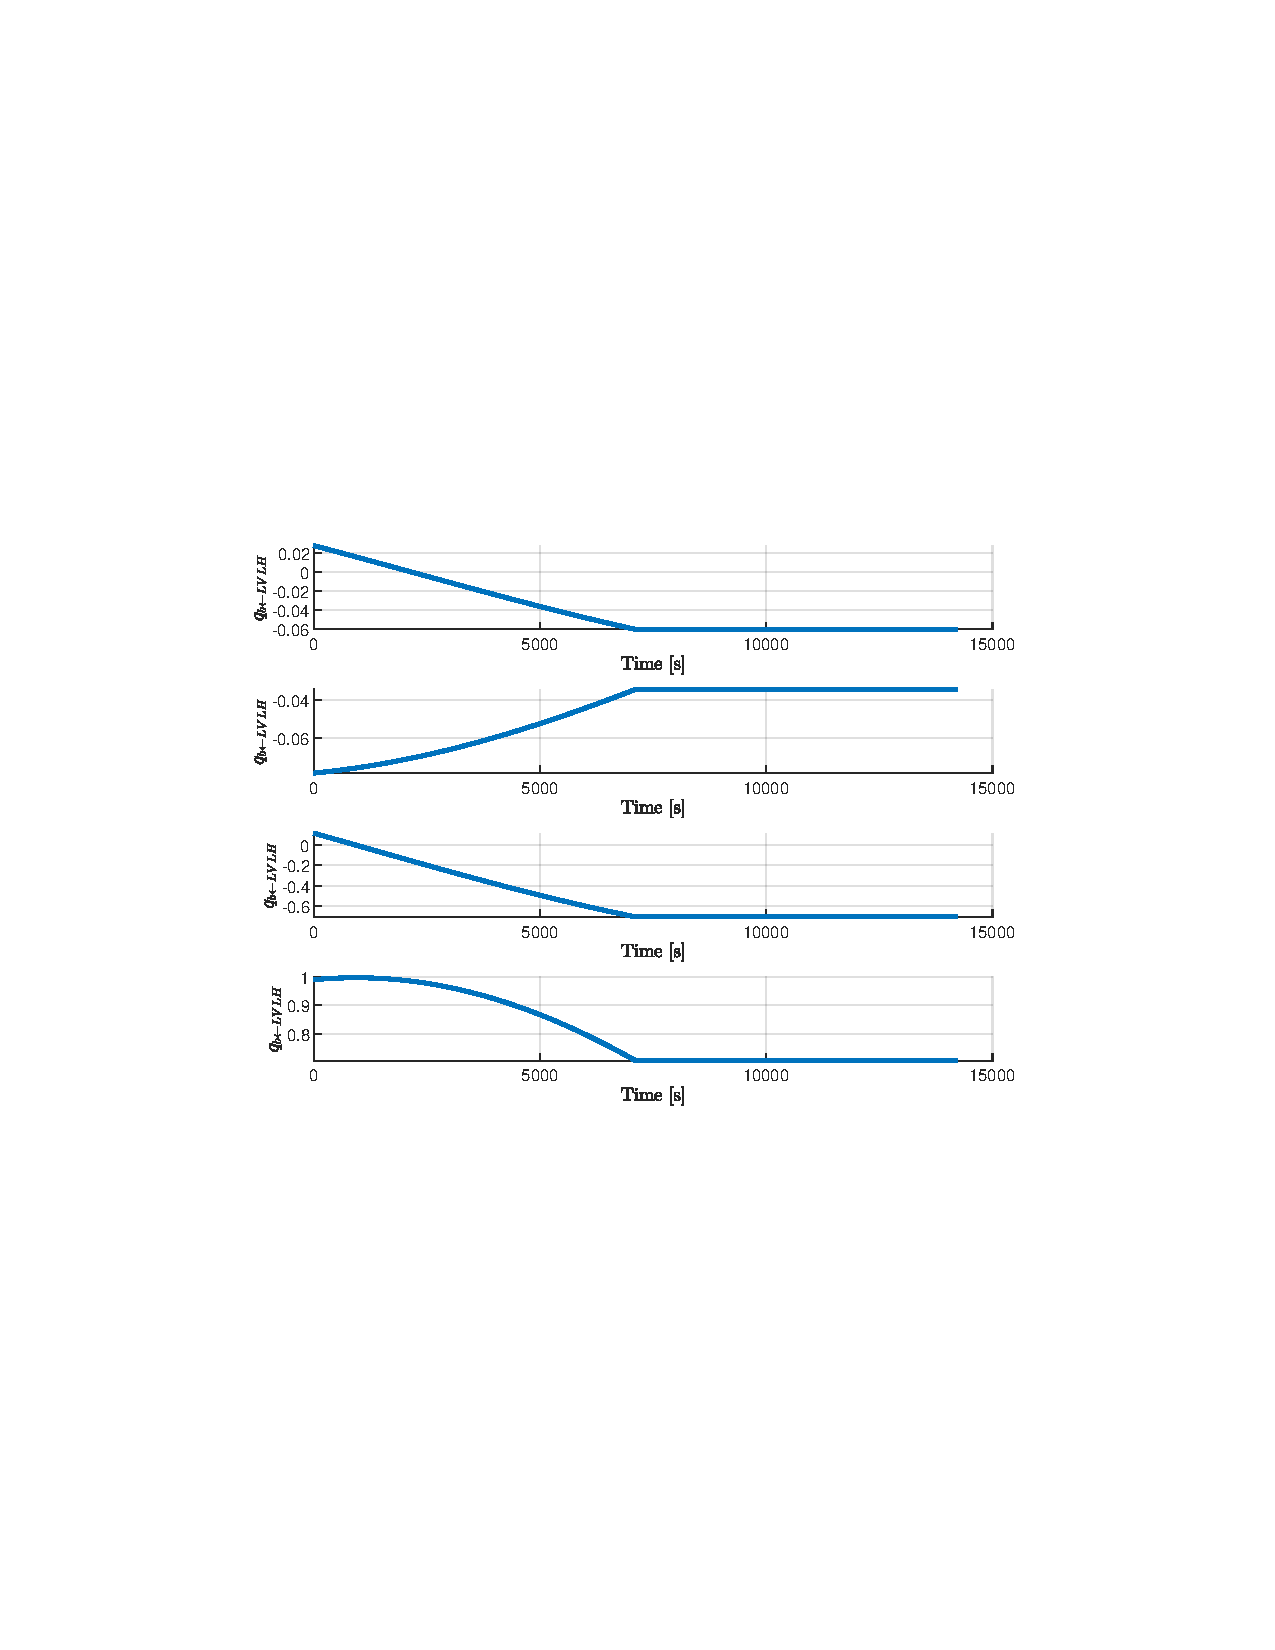
\includegraphics[width=\linewidth,trim={4cm, 8cm, 4cm, 8cm},clip]{figs/P1Q2.pdf}
	\caption{The nominal LVLH to body quaternion. Here we see that the quaternion is commanded to be constant at the end of the maneuver.}
	\label{fig:P1Q2}
\end{figure}

\begin{figure}[!h]
	\centering
	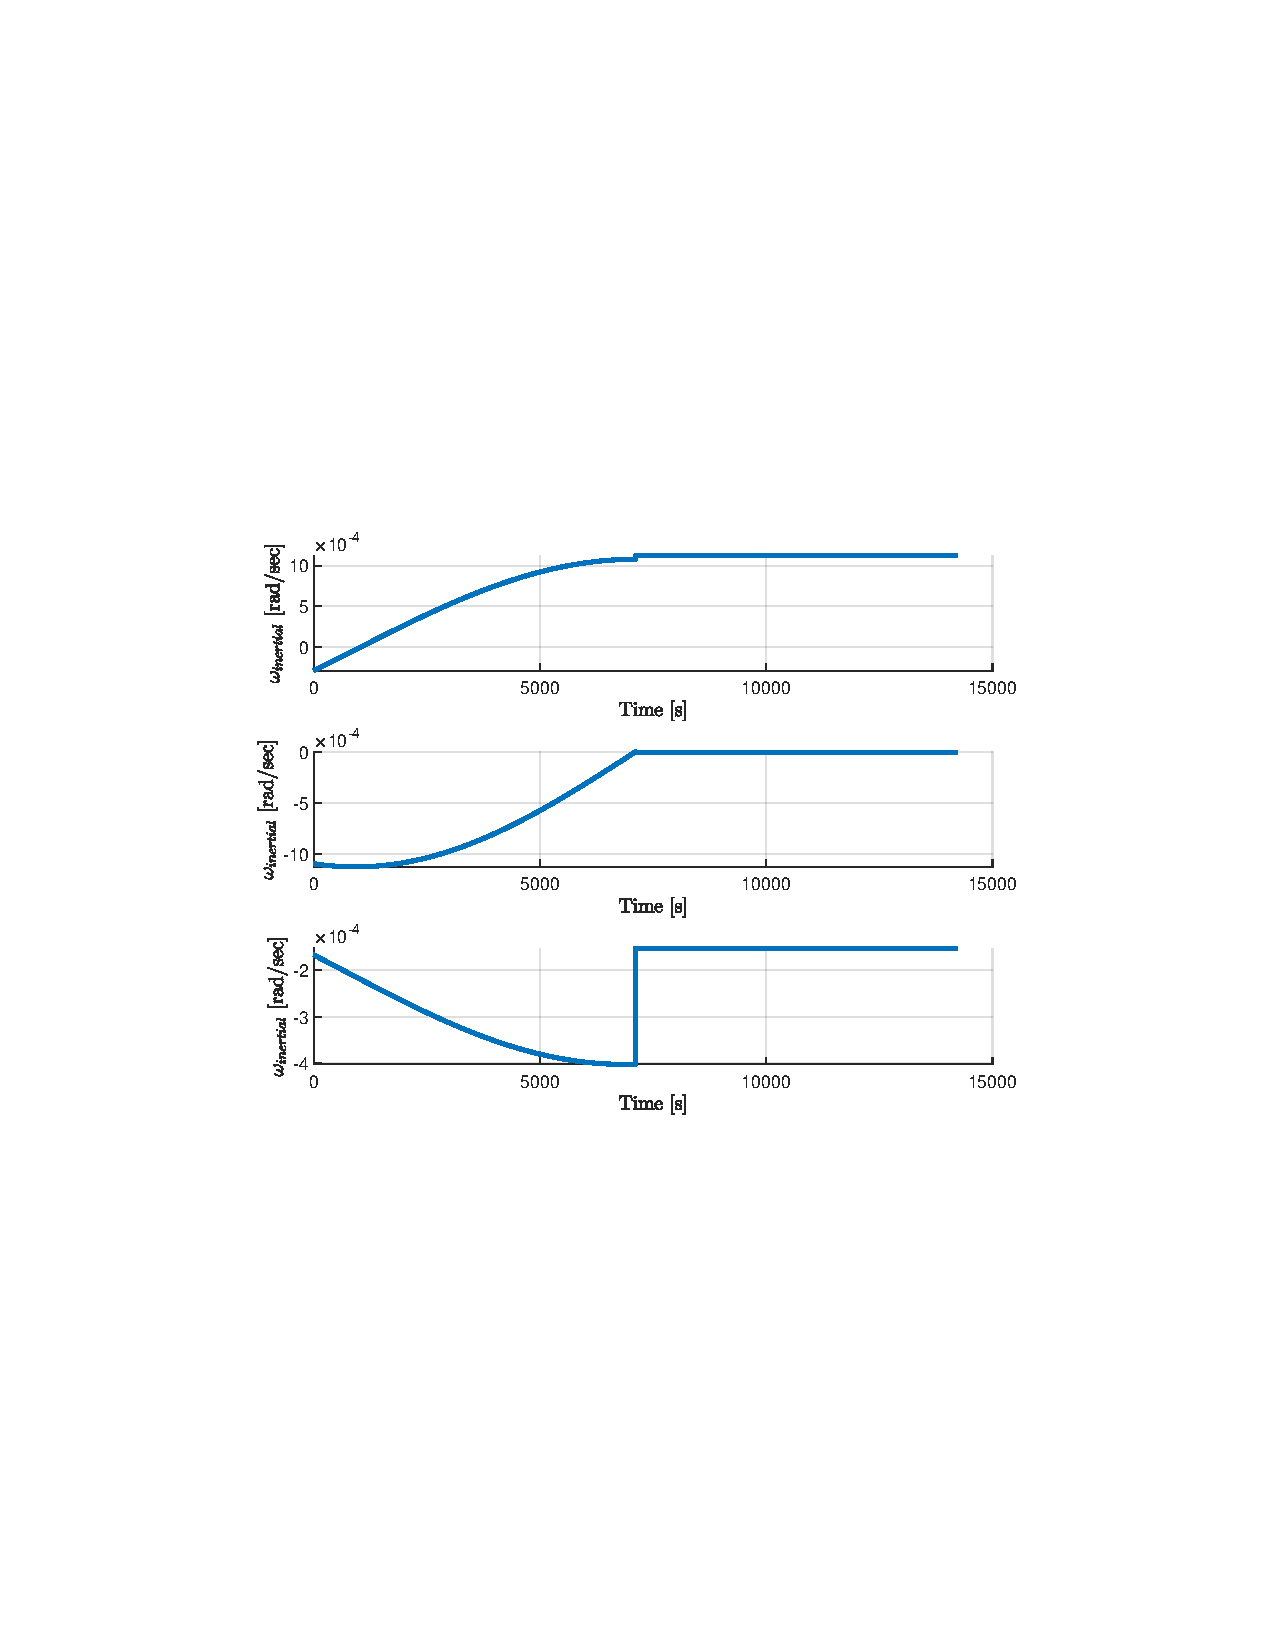
\includegraphics[width=\linewidth,trim={4cm, 8cm, 4cm, 8cm},clip]{figs/P1Q3.pdf}
	\caption{The nominal inertial to body angular rates. These are not zero after the maneuver because the LVLH frame is rotating.}
	\label{fig:P1Q3}
\end{figure}

\begin{figure}[!h]
	\centering
	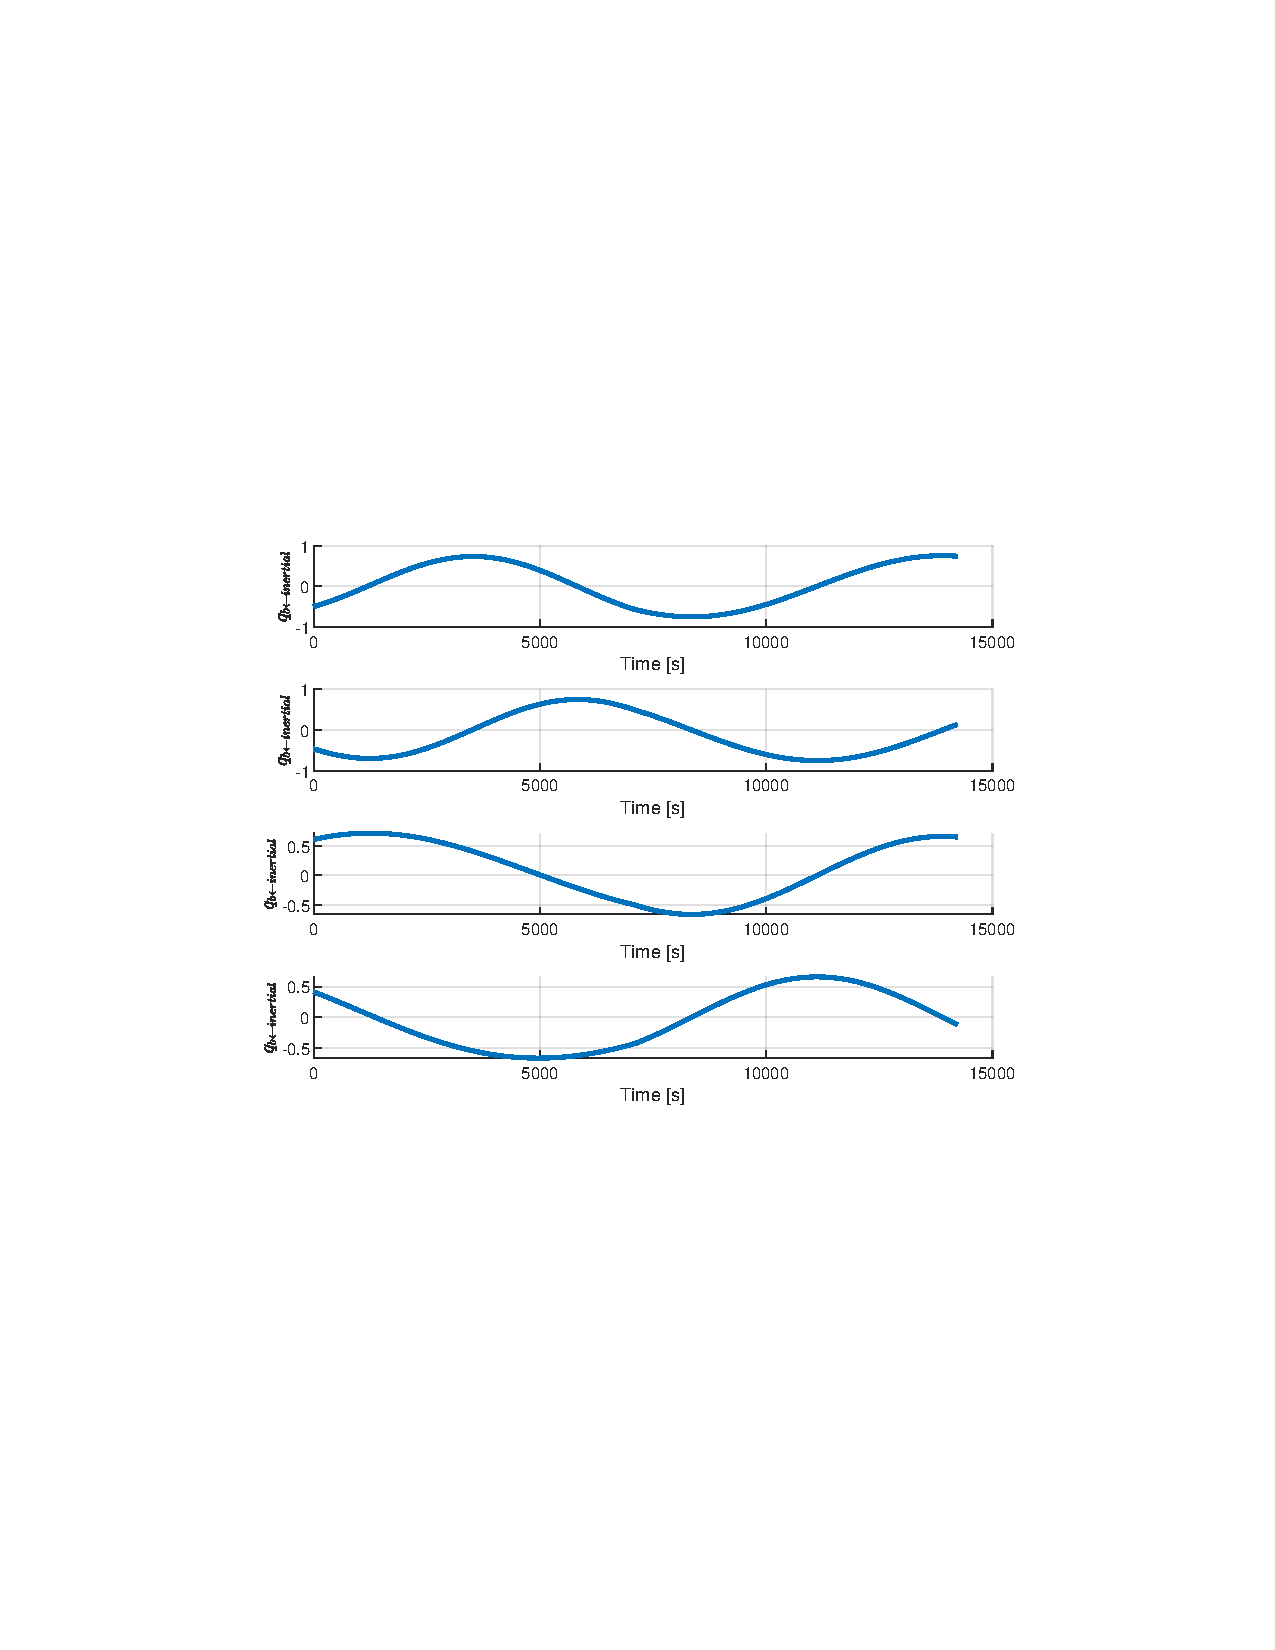
\includegraphics[width=\linewidth,trim={4cm, 8cm, 4cm, 8cm},clip]{figs/P1Q4.pdf}
	\caption{The nominal inertial to body quaternion. This is not constant after the maneuver because the LVLH frame is rotating.}
	\label{fig:P1Q4}
\end{figure}

\section{Part 2}

\begin{figure}[!h]
	\centering
	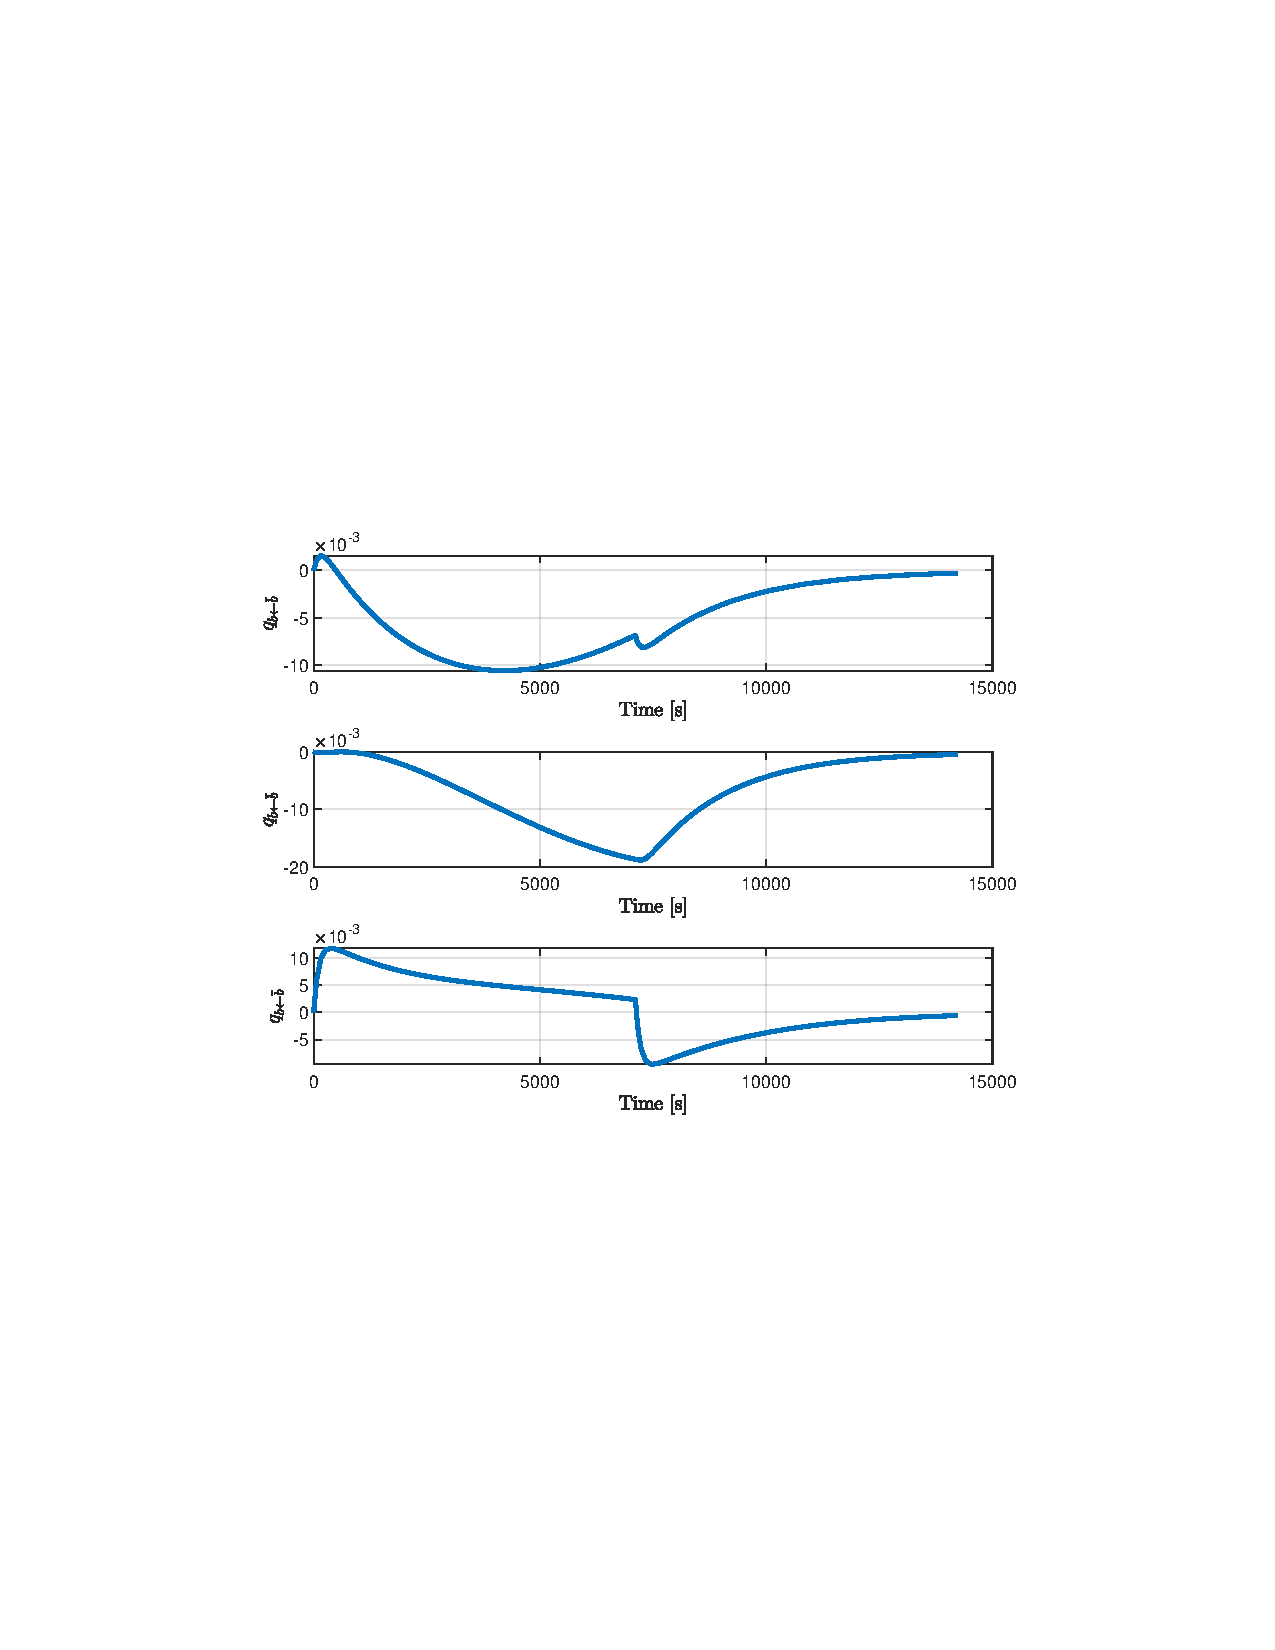
\includegraphics[width=\linewidth,trim={4cm, 8cm, 4cm, 8cm},clip]{figs/P2Q1.pdf}
	\caption{The attitude control error as represented by the vector components of the error quaternion. The commanded body rate profile is discontinuous at the beginning and end of the maneuver, resulting in overshoot and poor tracking performance after those moments.}
	\label{fig:P2Q1}
\end{figure}

\begin{figure}[!h]
	\centering
	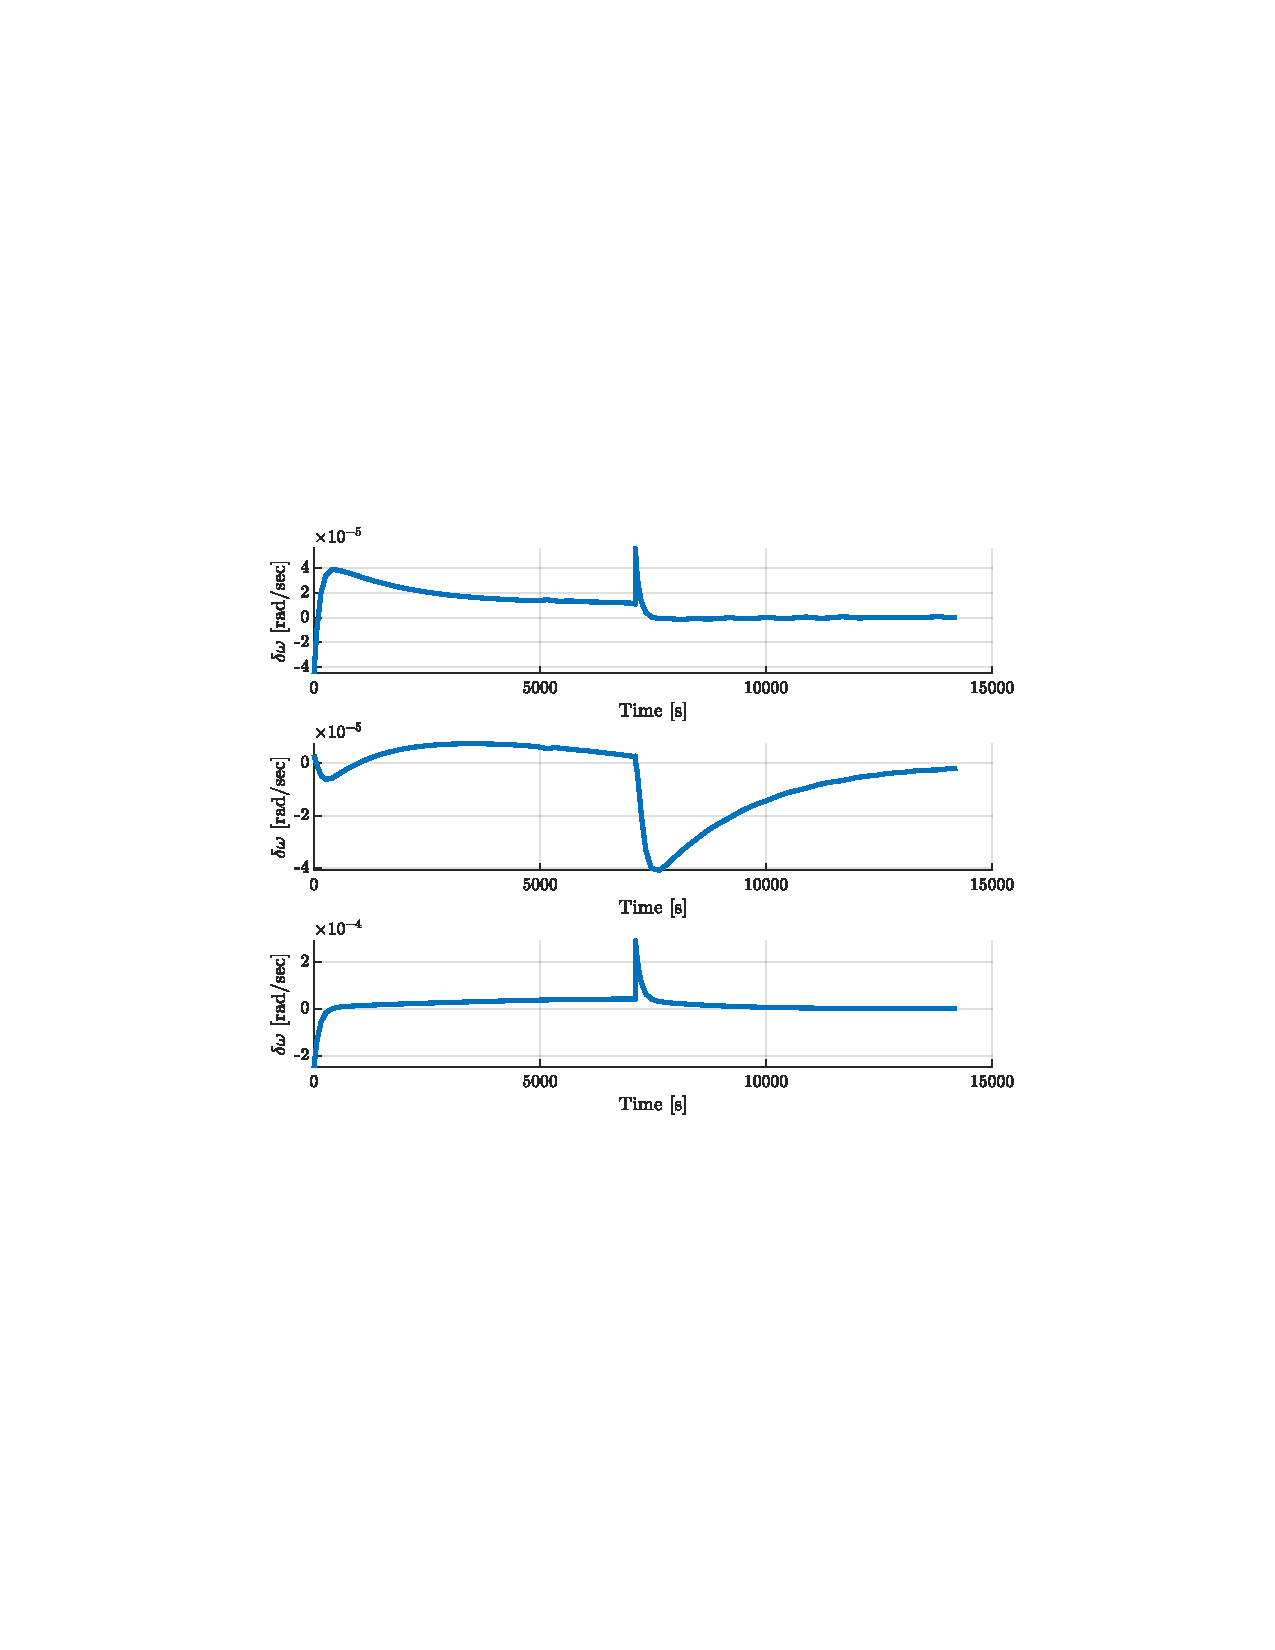
\includegraphics[width=\linewidth,trim={4cm, 8cm, 4cm, 8cm},clip]{figs/P2Q2.pdf}
	\caption{The attitude rate error. The commanded body rate profile is discontinuous at the beginning and end of the maneuver, resulting in overshoot and poor performance after those moments.}
	\label{fig:P2Q2}
\end{figure}

\begin{figure}[!h]
	\centering
	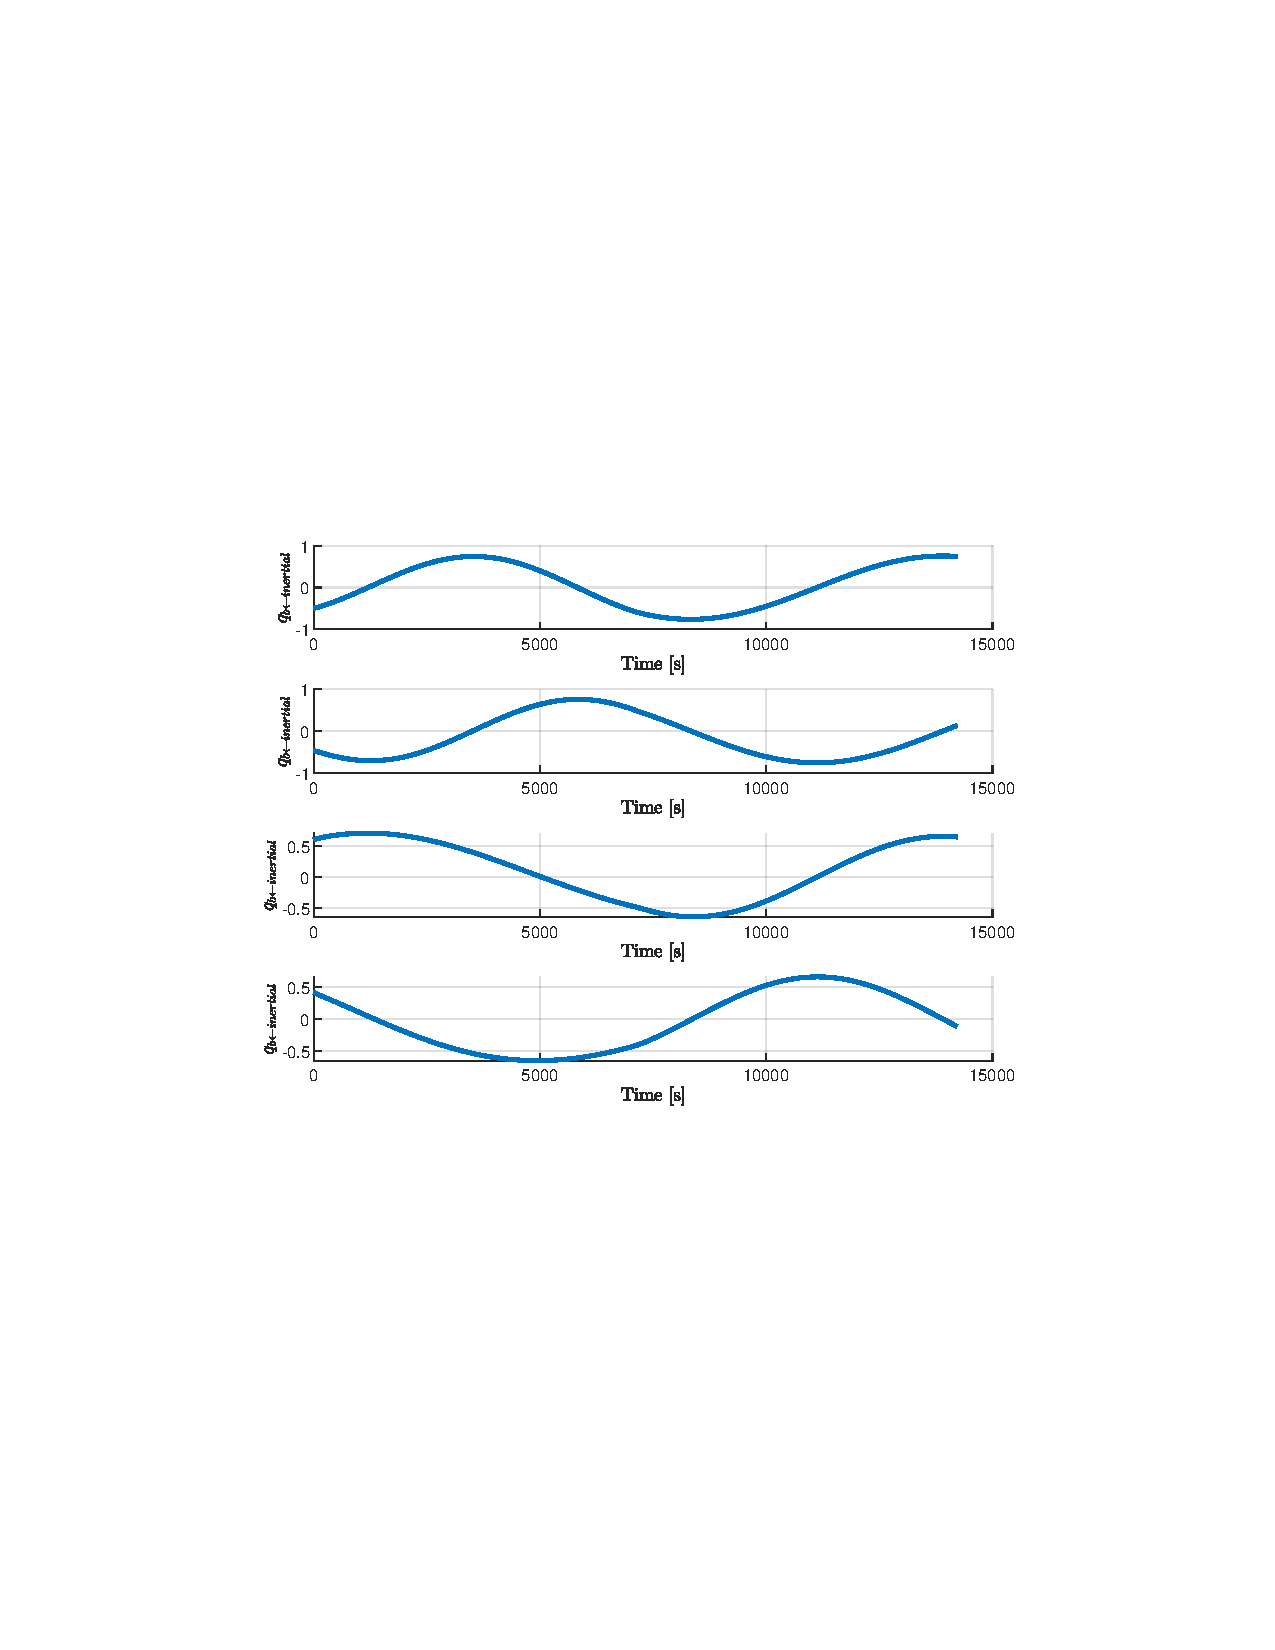
\includegraphics[width=\linewidth,trim={4cm, 8cm, 4cm, 8cm},clip]{figs/P2Q3.pdf}
	\caption{The true inertial to body quaternion.}
	\label{fig:P2Q3}
\end{figure}

\begin{figure}[!h]
	\centering
	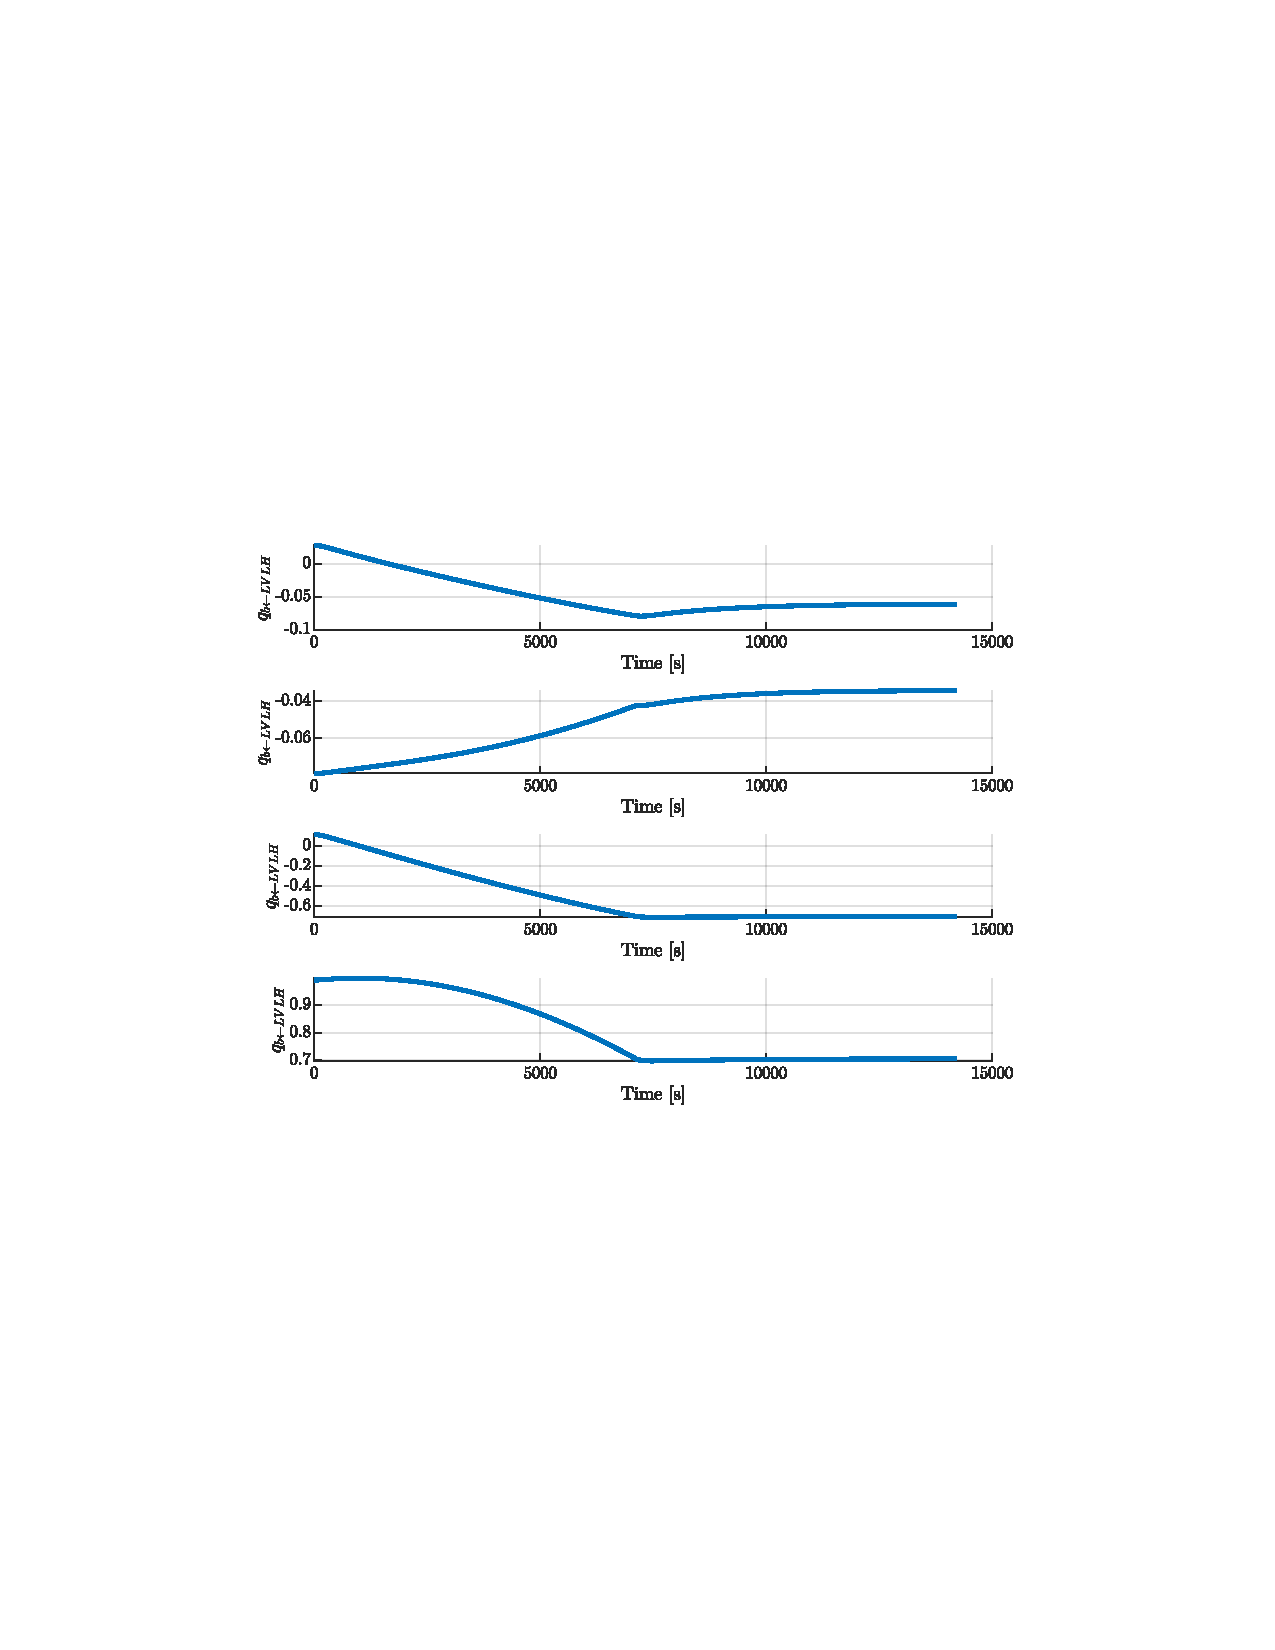
\includegraphics[width=\linewidth,trim={4cm, 8cm, 4cm, 8cm},clip]{figs/P2Q4.pdf}
	\caption{The true LVLH to body quaternion.}
	\label{fig:P2Q4}
\end{figure}

\section{Part 3}

\begin{figure}[!h]
	\centering
	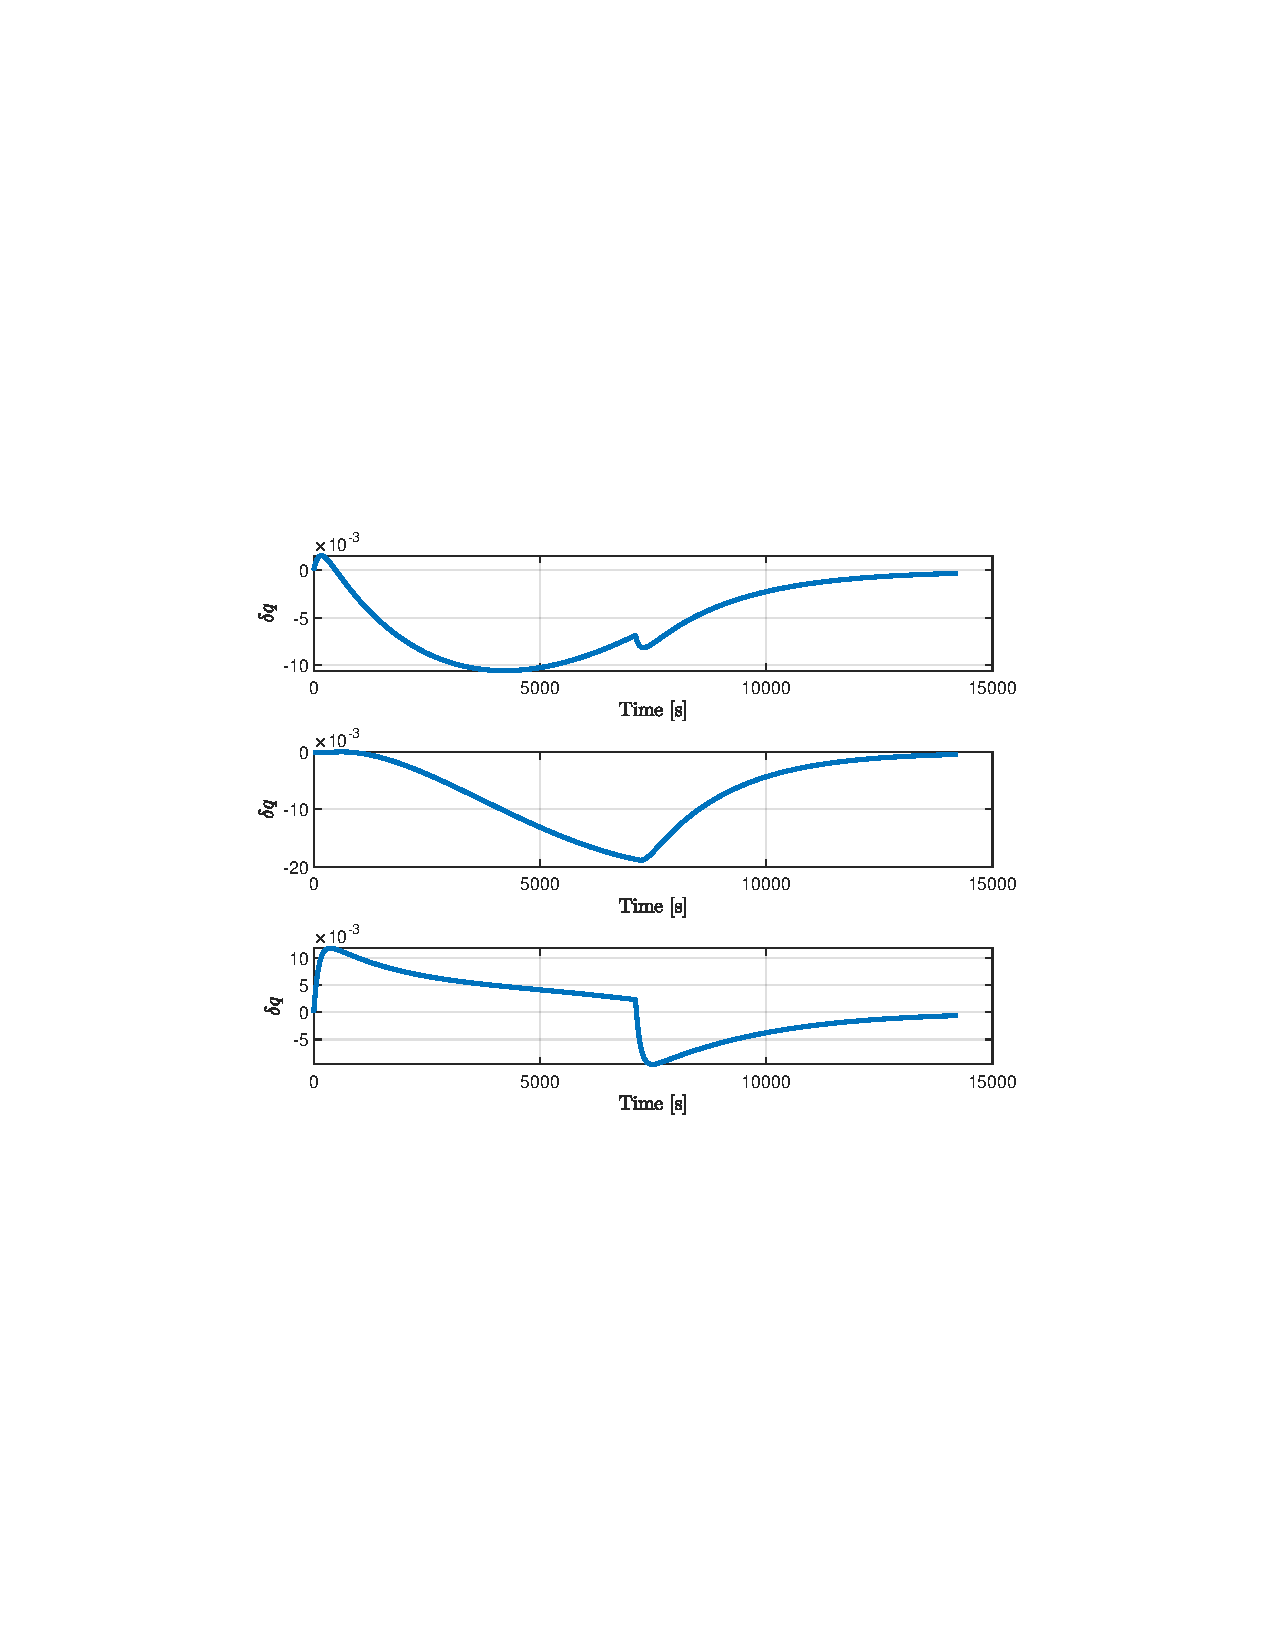
\includegraphics[width=\linewidth,trim={4cm, 8cm, 4cm, 8cm},clip]{figs/P3Q1.pdf}
	\caption{The attitude control error as represented by the vector components of the error quaternion. The commanded body rate profile is discontinuous at the beginning and end of the maneuver, resulting in overshoot and poor performance after those moments.}
	\label{fig:P3Q1}
\end{figure}

\begin{figure}[!h]
	\centering
	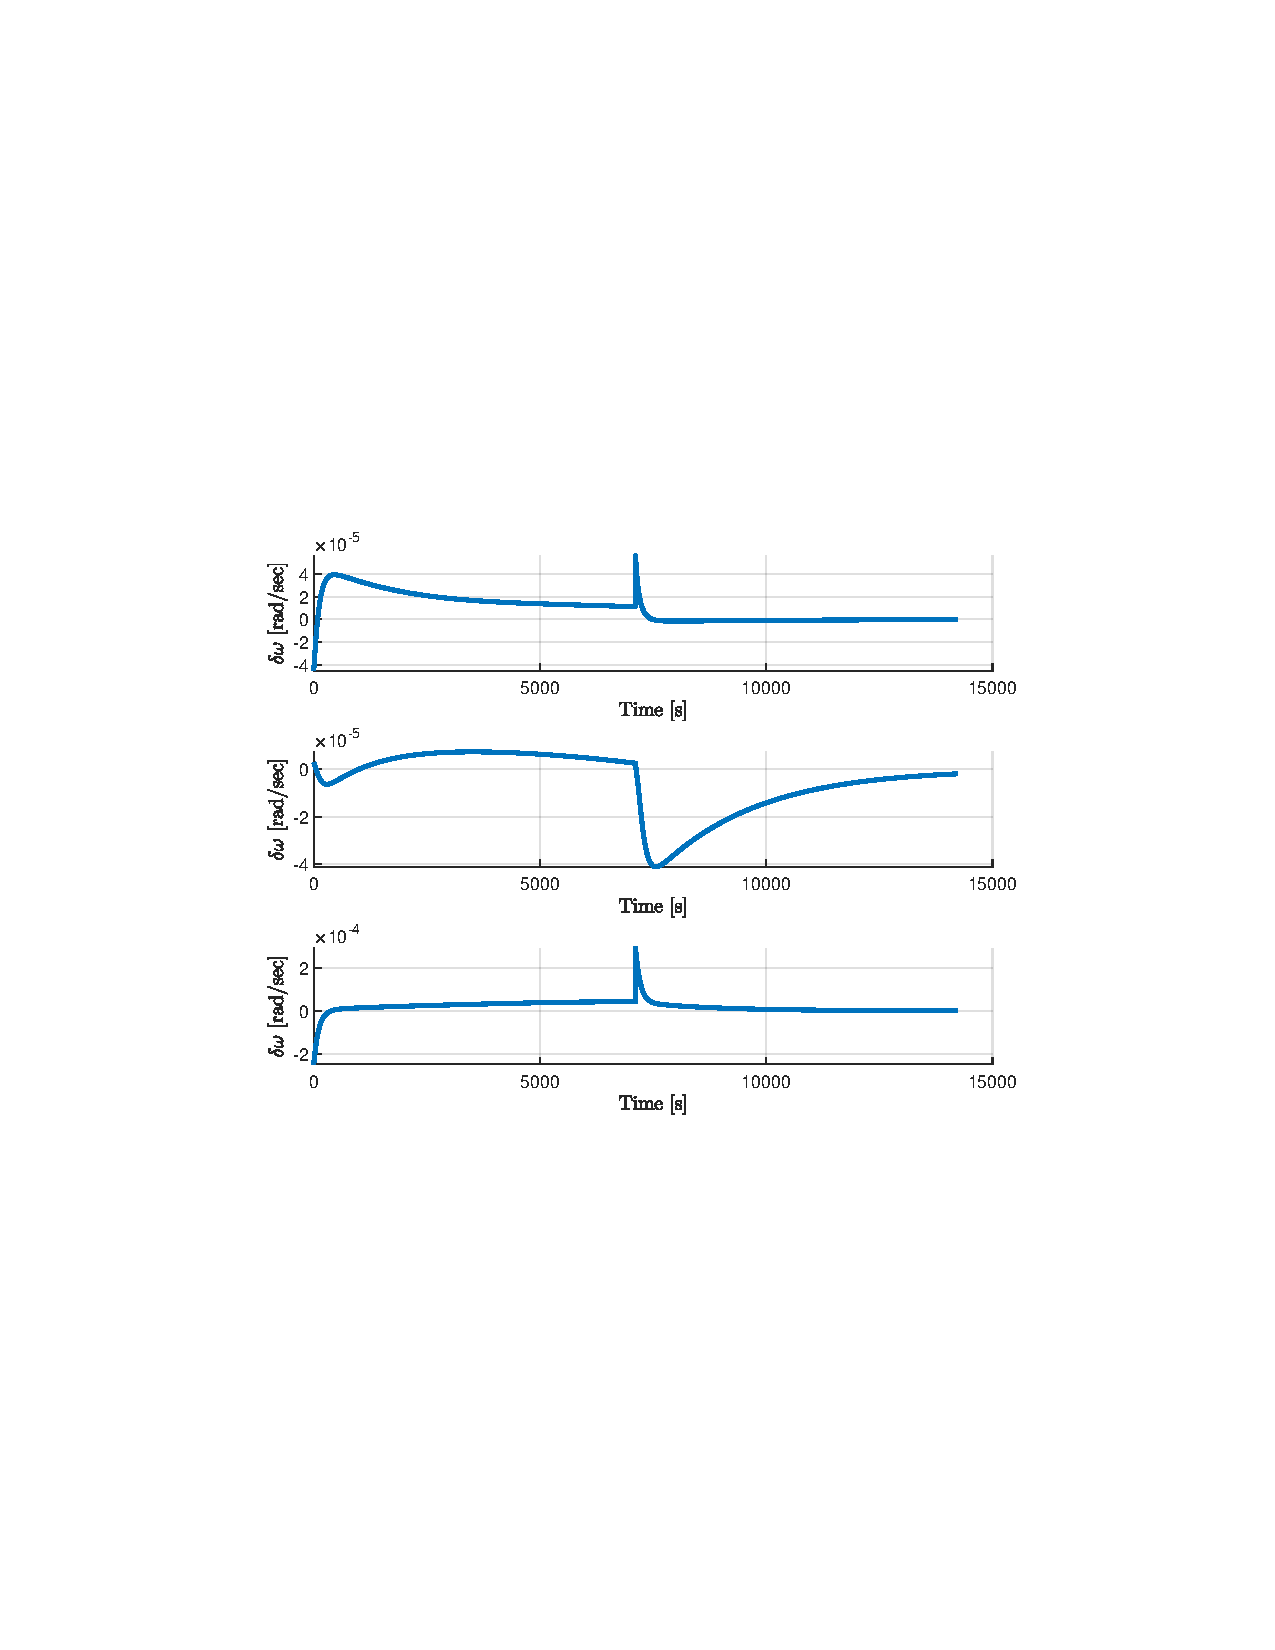
\includegraphics[width=\linewidth,trim={4cm, 8cm, 4cm, 8cm},clip]{figs/P3Q2.pdf}
	\caption{The attitude rate error. The commanded body rate profile is discontinuous at the beginning and end of the maneuver, resulting in overshoot and poor performance after those moments.}
	\label{fig:P3Q2}
\end{figure}

\begin{figure}[!h]
	\centering
	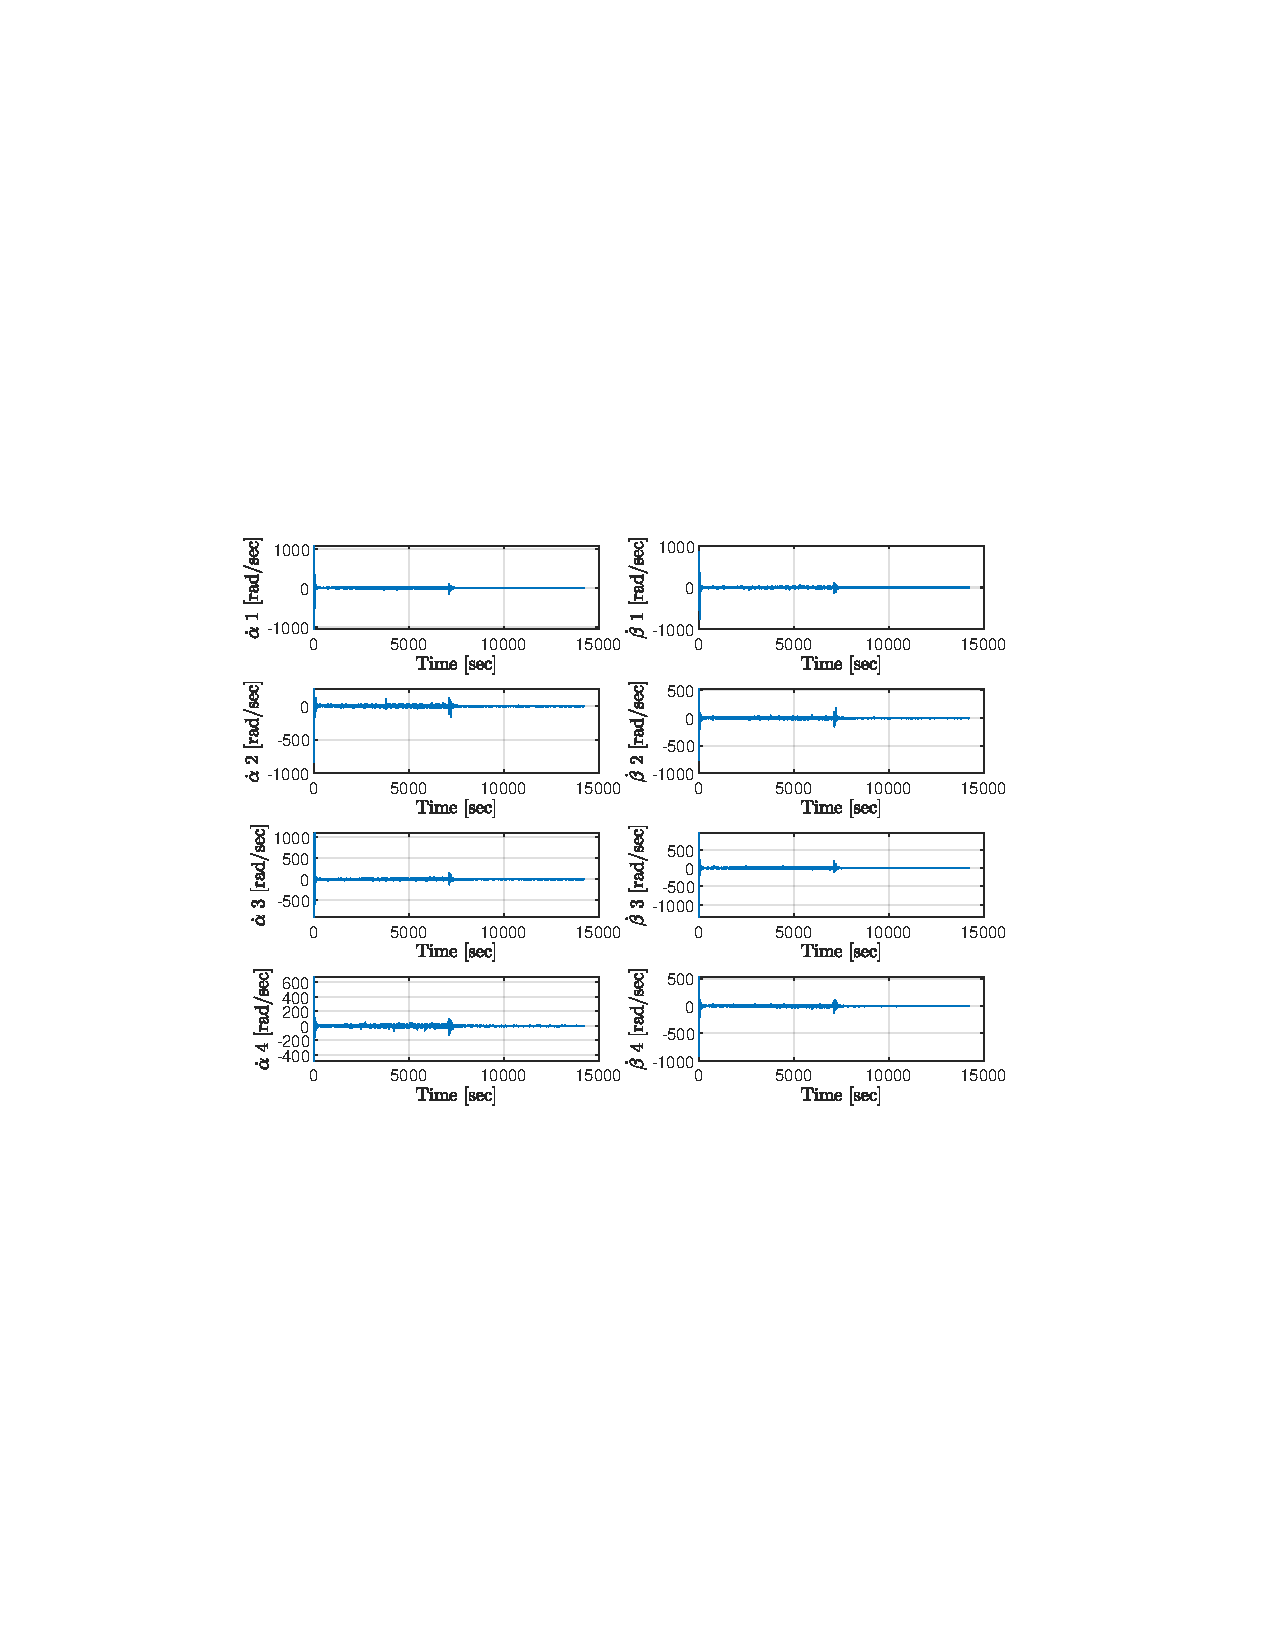
\includegraphics[width=\linewidth,trim={4cm, 8cm, 4cm, 8cm},clip]{figs/P3Q3.pdf}
	\caption{The gimbal rates for each CMG. These rates are extremely high and physically unrealizable. This occurs because our KD controller gains are very high and the system contains no logic to saturate the commanded gimbal rate.}
	\label{fig:P3Q3}
\end{figure}

\begin{figure}[!h]
	\centering
	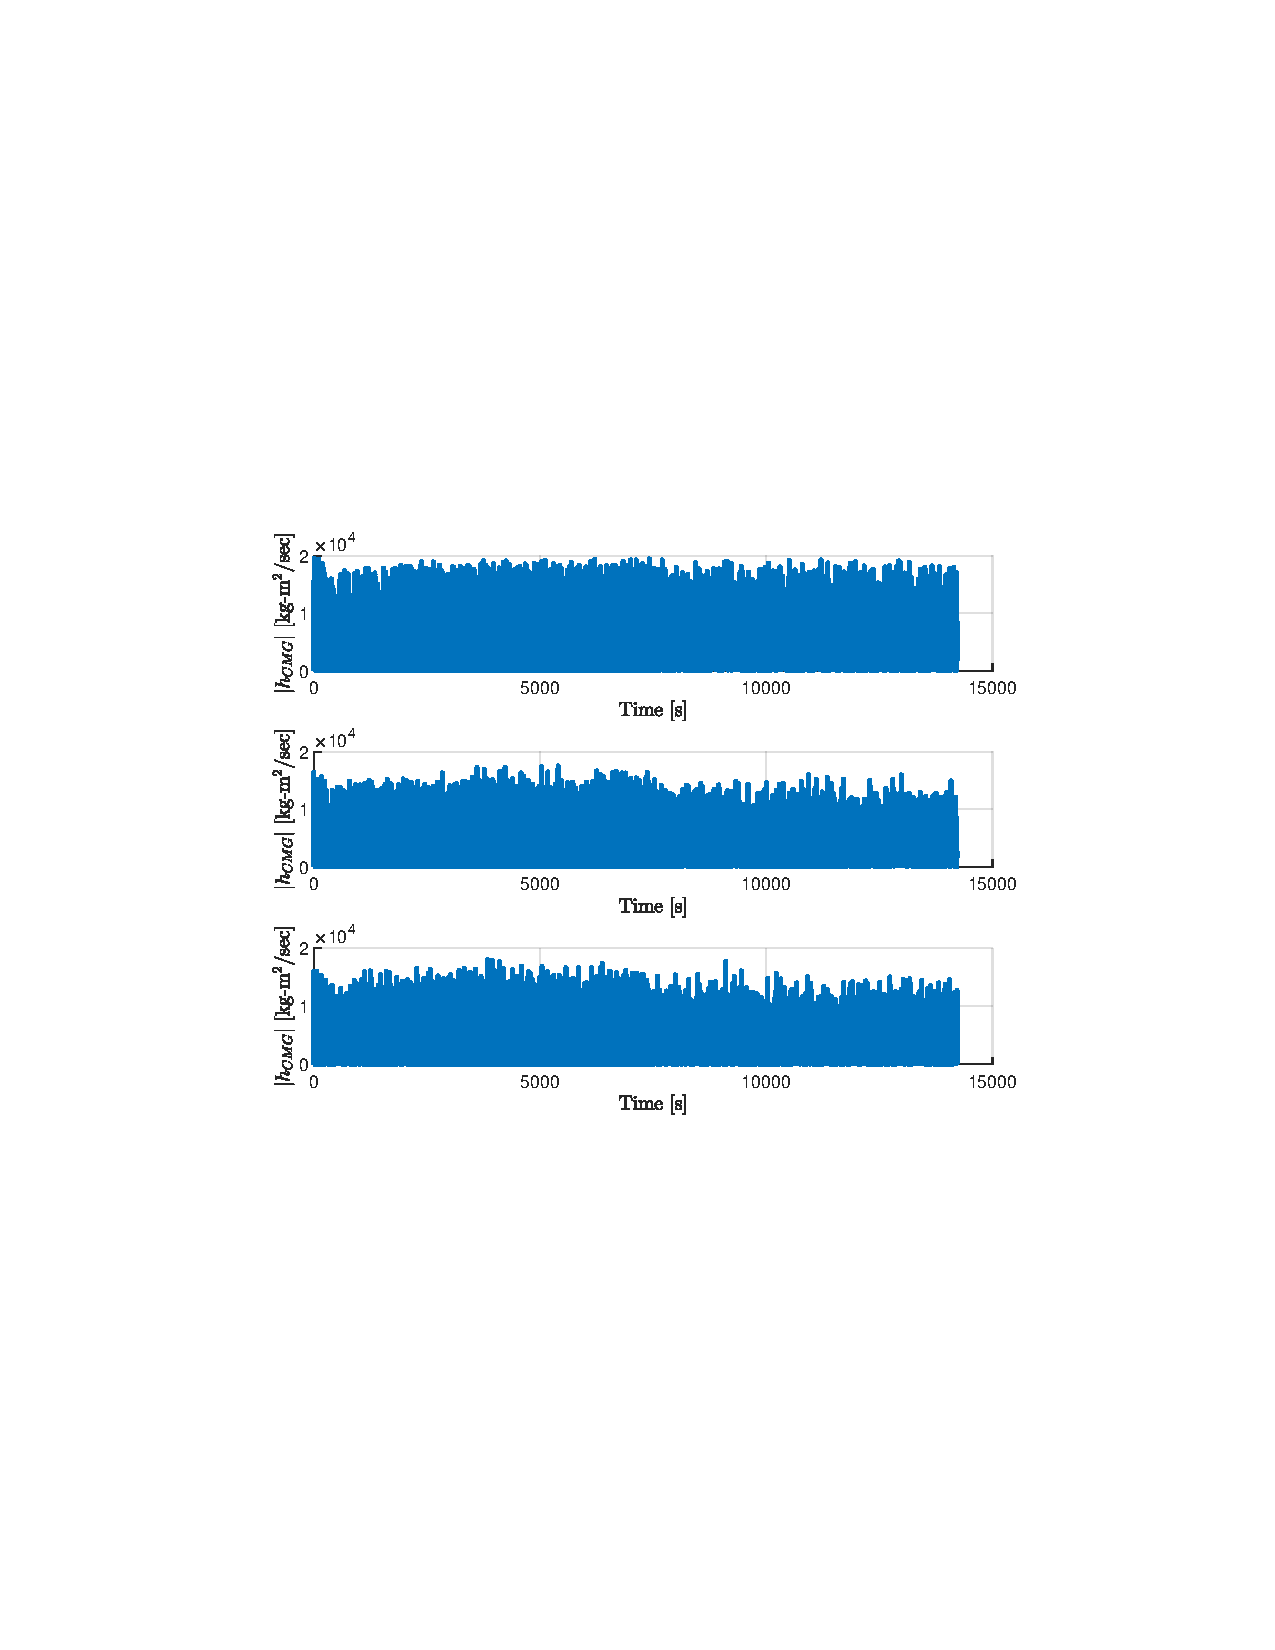
\includegraphics[width=\linewidth,trim={4cm, 8cm, 4cm, 8cm},clip]{figs/P3Q4.pdf}
	\caption{The magnitude of each element of the angular momentum vector for the CMG array. The rate of change of this vector is extremely high due to the physically unrealizable gimbal rates.}
	\label{fig:P3Q4}
\end{figure}

\begin{figure}[!h]
	\centering
	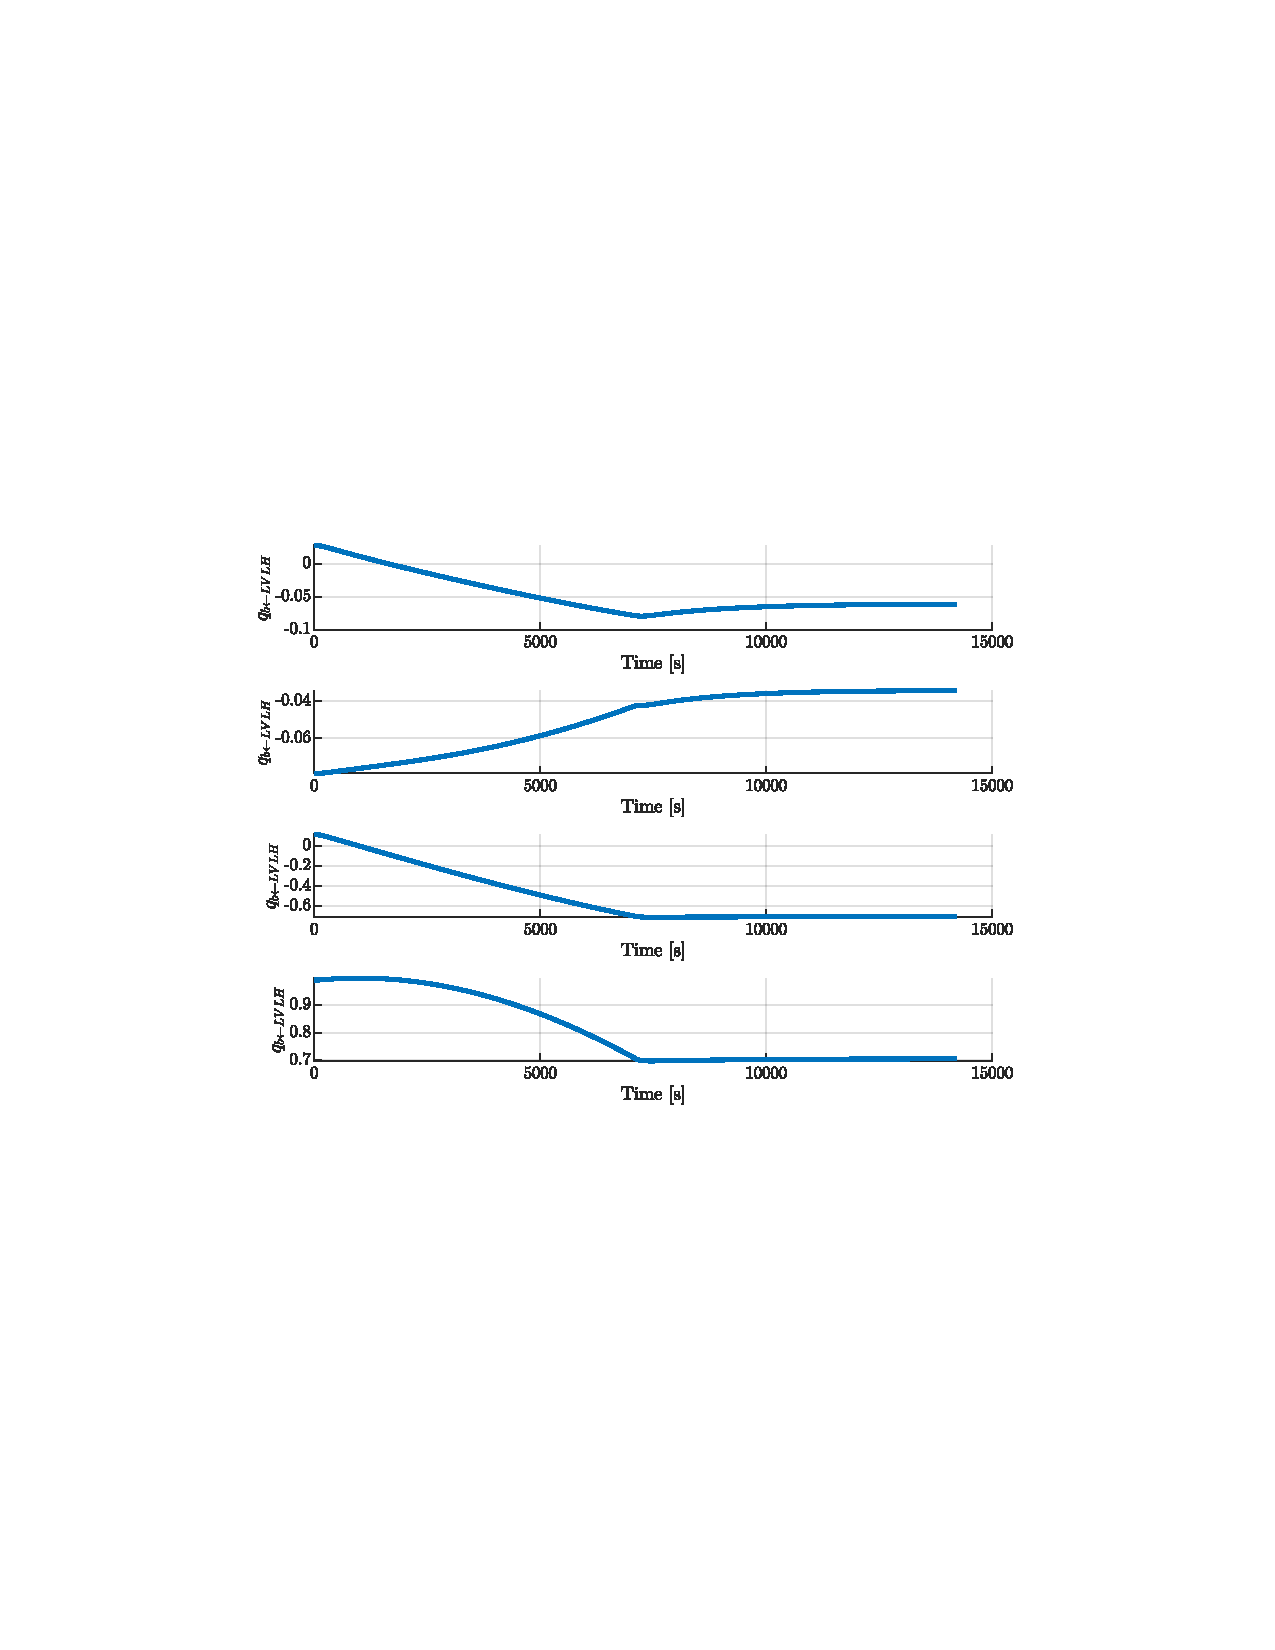
\includegraphics[width=\linewidth,trim={4cm, 8cm, 4cm, 8cm},clip]{figs/P3Q5.pdf}
	\caption{The true LVLH to body attitude quaternion.}
	\label{fig:P3Q5}
\end{figure}

\section{Code}

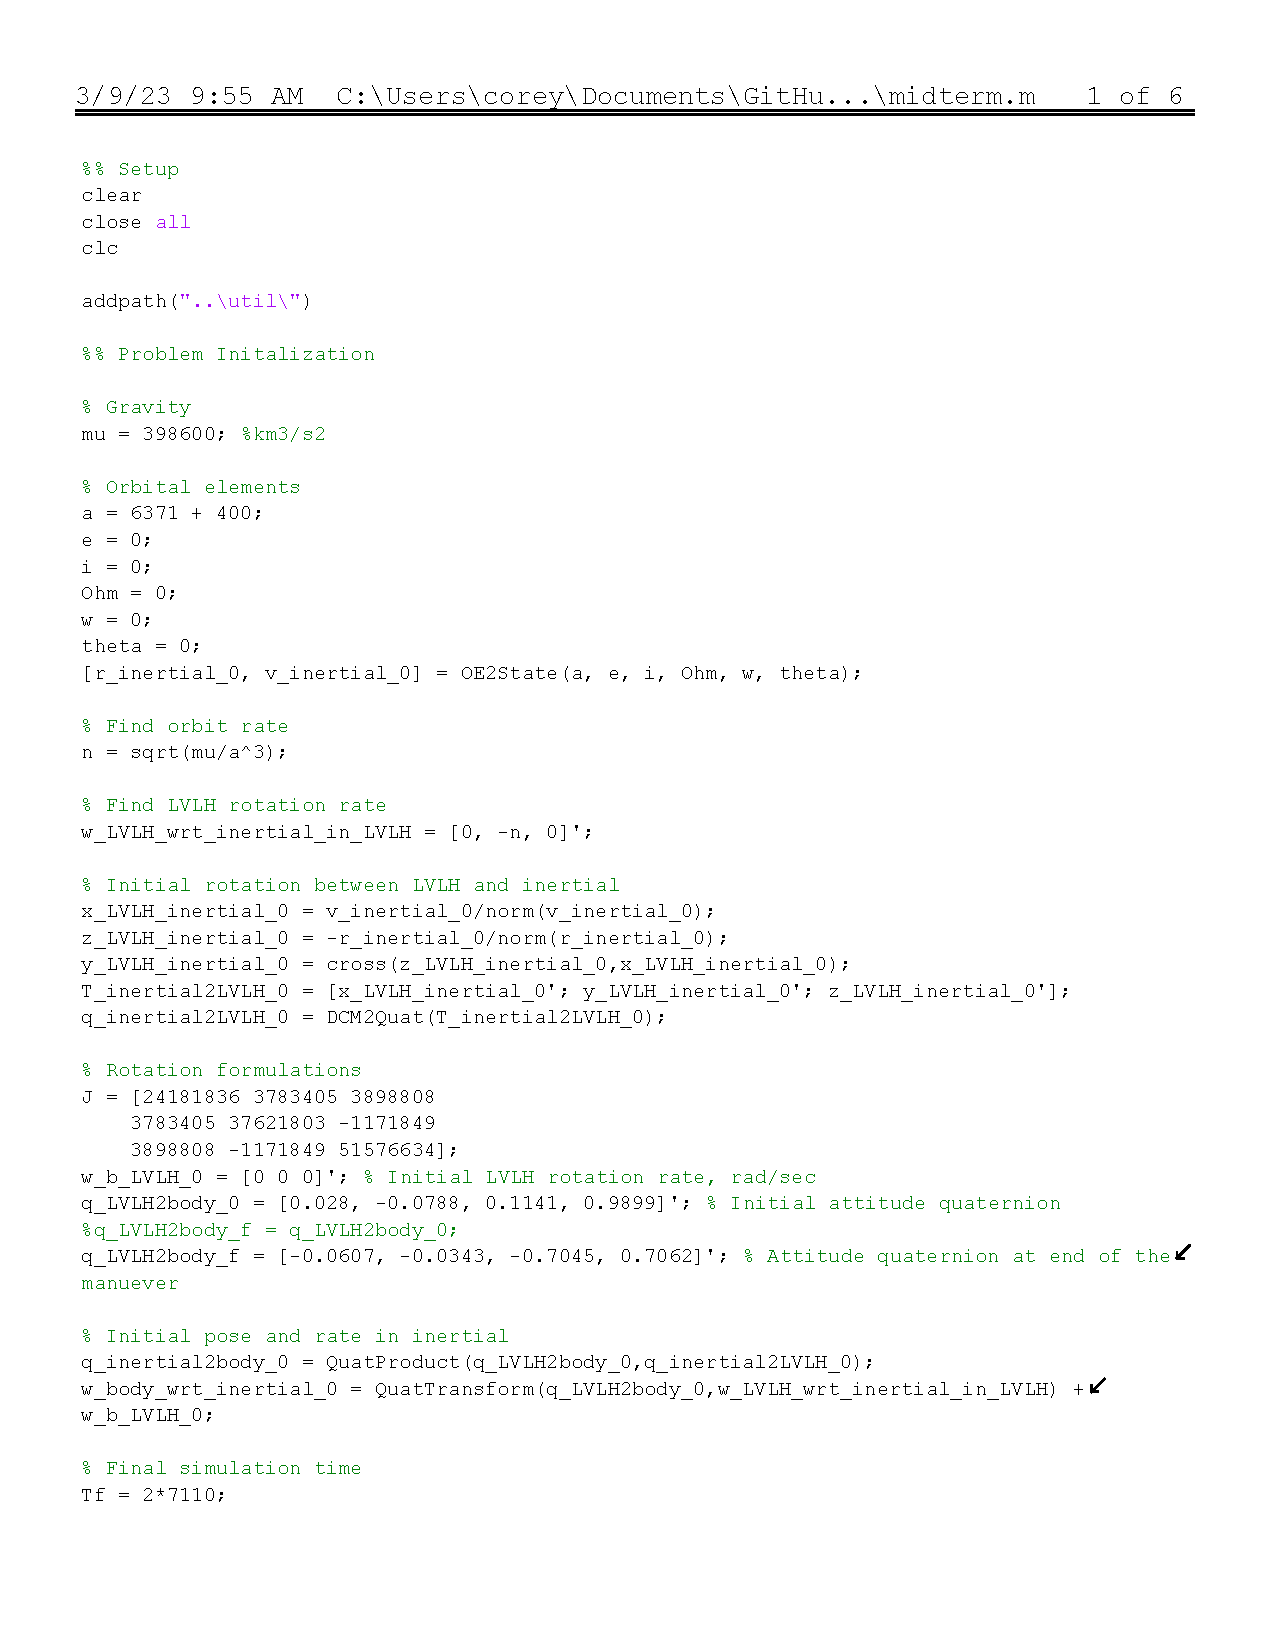
\includepdf[pages=-,pagecommand={},width=\textwidth]{code_main.pdf}
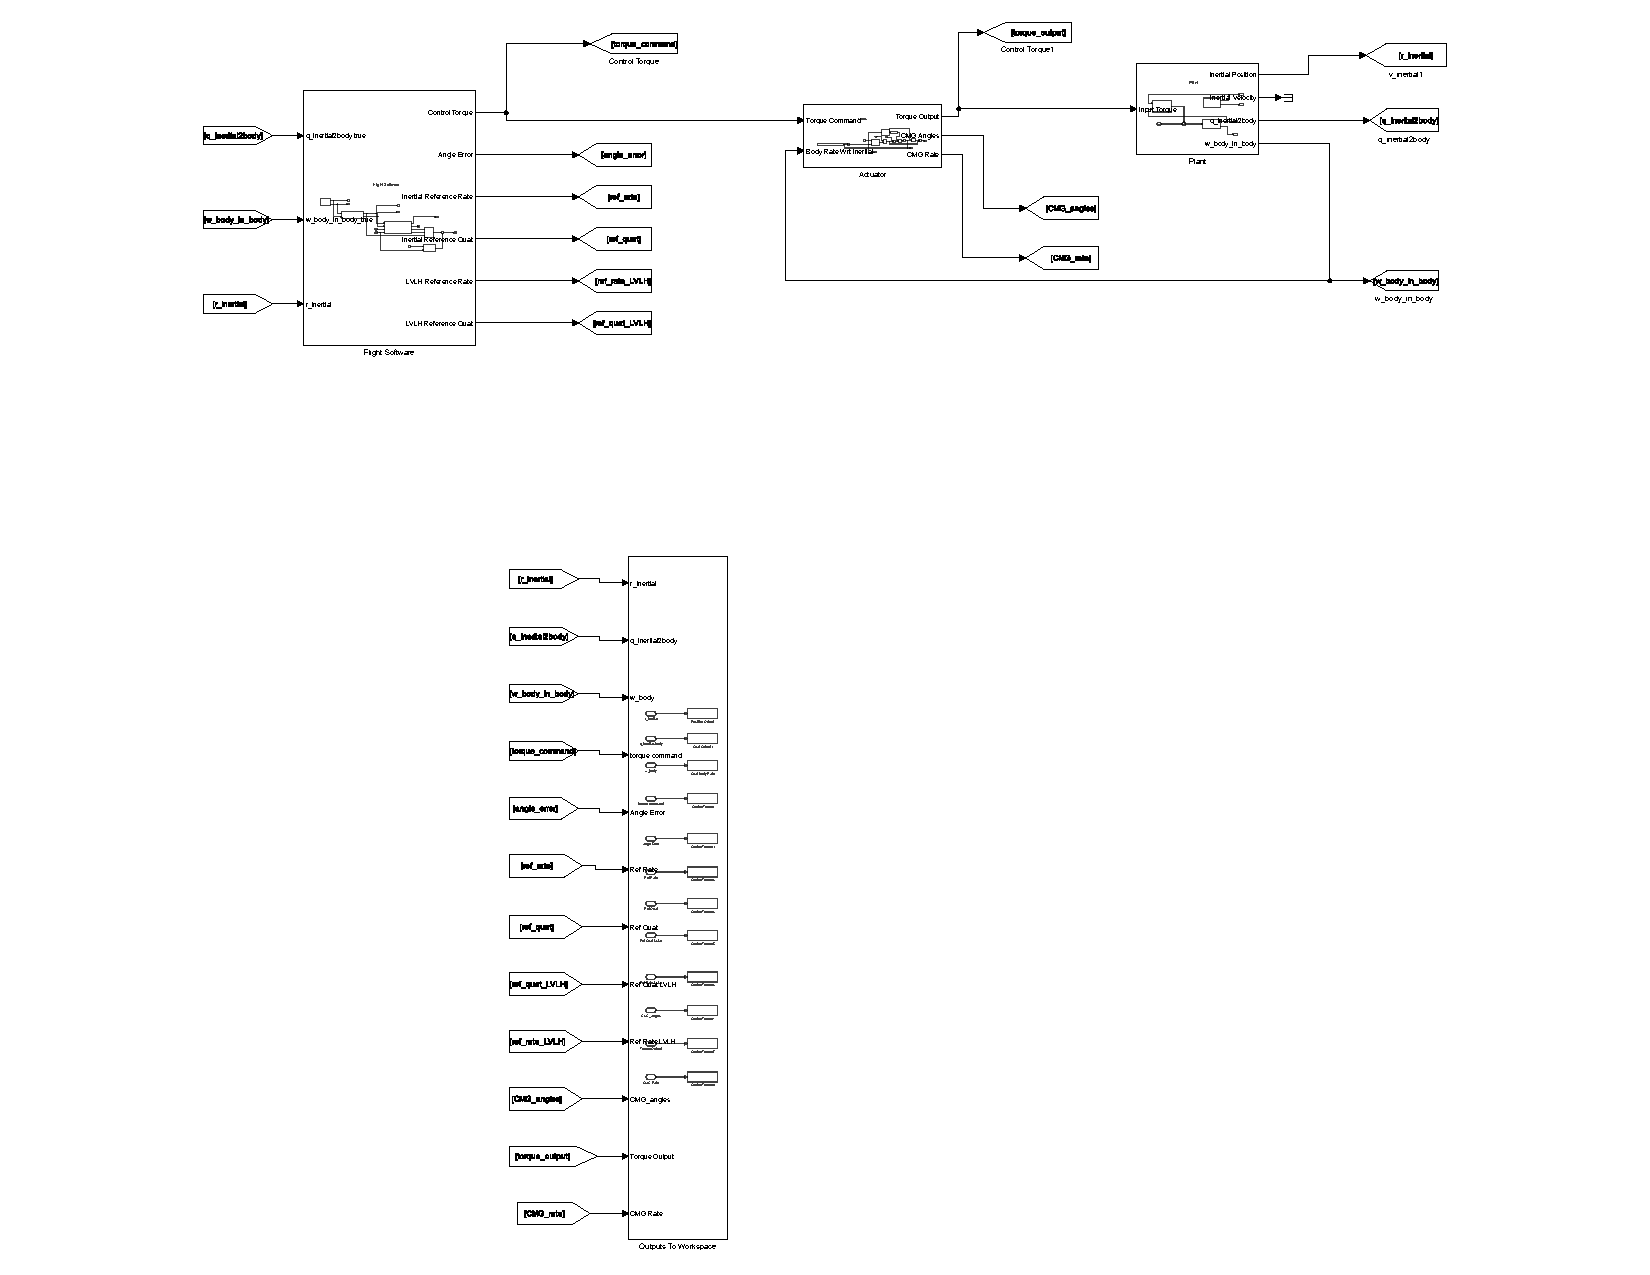
\includepdf[pages=-,pagecommand={},width=\textwidth]{../simulink/code_doc.pdf}

\end{document}
